\documentclass{article}
\usepackage{pgfplots}
\pgfplotsset{compat=1.18}

\begin{document}

\begin{figure}[ht]
\centering
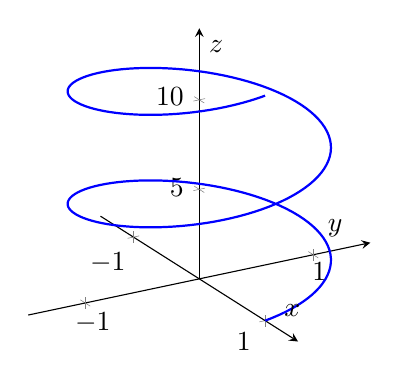
\begin{tikzpicture}
\begin{axis}[
    view={60}{30},
    axis lines=center,
    xlabel={$x$}, ylabel={$y$}, zlabel={$z$},
    xmin=-1.5, xmax=1.5,
    ymin=-1.5, ymax=1.5,
    zmin=0, zmax=14,
    xtick={-1,1}, ytick={-1,1}, ztick={5,10},
]
\addplot3[
    domain=0:4*pi,
    samples=200,
    samples y=0,
    variable=t,
    thick,
    blue,
] ({cos(deg(t))}, {sin(deg(t))}, {t});
\end{axis}
\end{tikzpicture}
\caption{A circular helix $\mathbf{r}(t) = (\cos t, \sin t, t)$.}
\end{figure}

\end{document}
